\documentclass[aspectratio=169,12pt,t]{beamer}

% --- Theme: Metropolis (modern, clean) ---
\usetheme[progressbar=frametitle,numbering=fraction,block=fill]{metropolis}

% --- Fira Sans font (install texlive-fonts-extra if missing) ---
\IfFileExists{FiraSans.sty}{\usepackage[sfdefault]{FiraSans}}{}

% --- Light background with warm accent ---
\definecolor{mDarkTeal}{RGB}{35,55,59}
\definecolor{mLightBrown}{RGB}{235,228,216}
\definecolor{mAccent}{RGB}{140,70,20}

\setbeamercolor{normal text}{fg=mDarkTeal,bg=white}
\setbeamercolor{alerted text}{fg=mAccent}
\setbeamercolor{frametitle}{bg=mDarkTeal,fg=white}
\setbeamercolor{progress bar}{fg=mAccent,bg=mLightBrown}
\setbeamercolor{title separator}{fg=mAccent}
\setbeamercolor{progress bar in head/foot}{fg=mAccent,bg=mLightBrown}
\setbeamercolor{progress bar in section page}{fg=mAccent,bg=mLightBrown}

% --- Packages ---
\usepackage[utf8]{inputenc}
\usepackage{amsmath,amssymb,amsthm}
\usepackage{mathrsfs}
\usepackage{tikz}
\usetikzlibrary{arrows.meta,positioning,calc,decorations.pathreplacing,shapes,patterns}
\usepackage{enumitem}
\usepackage{pgfplots}
\pgfplotsset{compat=1.18}

% --- Custom colors for content types ---
\definecolor{defcolor}{RGB}{25,85,120}
\definecolor{thmcolor}{RGB}{140,35,35}
\definecolor{proofcolor}{RGB}{35,100,50}
\definecolor{excolor}{RGB}{140,75,10}
\definecolor{remcolor}{RGB}{90,90,90}

% --- Beamer blocks for mathematical content types ---
\newenvironment{defblock}[1]{%
  \setbeamercolor{block title}{bg=defcolor,fg=white}%
  \setbeamercolor{block body}{bg=defcolor!5}%
  \begin{block}{#1}}{\end{block}}

\newenvironment{thmblock}[1]{%
  \setbeamercolor{block title}{bg=thmcolor,fg=white}%
  \setbeamercolor{block body}{bg=thmcolor!5}%
  \begin{block}{#1}}{\end{block}}

\newenvironment{proofblock}[1]{%
  \setbeamercolor{block title}{bg=proofcolor,fg=white}%
  \setbeamercolor{block body}{bg=proofcolor!5}%
  \begin{block}{#1}}{\end{block}}

\newenvironment{exblock}[1]{%
  \setbeamercolor{block title}{bg=excolor,fg=white}%
  \setbeamercolor{block body}{bg=excolor!5}%
  \begin{block}{#1}}{\end{block}}

\newenvironment{remblock}[1]{%
  \setbeamercolor{block title}{bg=remcolor,fg=white}%
  \setbeamercolor{block body}{bg=remcolor!5}%
  \begin{block}{#1}}{\end{block}}

% --- Metadata ---
\title{Chapter 1: The Real and Complex Number Systems}
\subtitle{Section: Fields}
\author{Based on Walter Rudin's \emph{Principles of Mathematical Analysis}}
\date{}

\begin{document}

% =============================================================================
% TITLE AND OUTLINE
% =============================================================================

\begin{frame}
  \titlepage
  \note{
    Welcome to Chapter 1, Section 3: Fields. In this section, we introduce
    the algebraic structure known as a field. Fields give us the precise
    rules for addition and multiplication that underlie the real numbers,
    the rationals, and the complex numbers. We will also define ordered
    fields, which combine algebraic and order structure. Let's get started.
  }
\end{frame}

\begin{frame}{Outline}
  \tableofcontents
  \note{
    Here is our roadmap for this section. We will begin with the definition
    of a field and its axioms, then explore the immediate consequences of
    those axioms. After that, we will introduce ordered fields and prove
    the basic properties of inequalities. Let's dive in.
  }
\end{frame}

% =============================================================================
% SECTION: INTRODUCTION AND MOTIVATION
% =============================================================================

\section{Motivation}

% --- Build 1/3 ---
\begin{frame}{Why This Section Matters}
  \begin{itemize}
    \item We need a \alert{precise algebraic framework} for the number systems used in analysis
  \end{itemize}

  \note{
    Before we can do analysis, we need to know exactly what operations are
    available and what rules they follow. The concept of a field gives us
    this precise algebraic framework. It captures the essential properties
    of addition and multiplication.
  }
\end{frame}

% --- Build 2/3 ---
\begin{frame}{Why This Section Matters}
  \begin{itemize}
    \item We need a \alert{precise algebraic framework} for the number systems used in analysis
    \item The rationals $\mathbb{Q}$, the reals $\mathbb{R}$, and the complex numbers $\mathbb{C}$ are all \emph{fields}
  \end{itemize}

  \note{
    The rationals, the reals, and the complex numbers all share the same
    basic algebraic structure. By proving results at the level of fields,
    we prove them once and for all, rather than repeating the work for each
    number system separately.
  }
\end{frame}

% --- Build 3/3 ---
\begin{frame}{Why This Section Matters}
  \begin{itemize}
    \item We need a \alert{precise algebraic framework} for the number systems used in analysis
    \item The rationals $\mathbb{Q}$, the reals $\mathbb{R}$, and the complex numbers $\mathbb{C}$ are all \emph{fields}
    \item Adding \emph{order} to a field gives an \alert{ordered field} --- the setting for inequalities
  \end{itemize}

  \note{
    Finally, we will combine the algebraic structure of a field with the
    order structure from the previous section to get an ordered field.
    Ordered fields are where inequalities live, and they provide the
    natural setting for the real number system. Let's begin with the
    definition of a field.
  }
\end{frame}

% =============================================================================
% SECTION: THE FIELD AXIOMS
% =============================================================================

\section{The Field Axioms}

% --- Definition 1.12: Introduction ---
\begin{frame}{Definition 1.12: Field}
  \begin{defblock}{Definition 1.12}
    A \alert{field} is a set $F$ with two operations, \emph{addition} and \emph{multiplication}, satisfying three groups of axioms:

    \vspace{0.5em}
    \begin{description}[labelwidth=2.6em, leftmargin=3.2em, font=\bfseries]
      \item[(A)] Axioms for addition
      \item[(M)] Axioms for multiplication
      \item[(D)] The distributive law
    \end{description}
  \end{defblock}

  \note{
    A field is a set equipped with two operations, addition and multiplication,
    that satisfy a specific list of axioms. These axioms are organized into
    three groups: the addition axioms, the multiplication axioms, and the
    distributive law that links the two operations together. Let's look at
    each group in turn.
  }
\end{frame}

% --- Addition Axioms: Build 1/3 ---
\begin{frame}{Definition 1.12: Axioms for Addition}
  \begin{defblock}{(A) Axioms for Addition}
    \begin{description}[labelwidth=2.6em, leftmargin=3.2em, font=\bfseries]
      \item[(A1)] If $x, y \in F$, then $x + y \in F$ \hfill\emph{(closure)}
      \item[(A2)] $x + y = y + x$ \hfill\emph{(commutativity)}
    \end{description}
  \end{defblock}

  \note{
    The first two addition axioms are closure and commutativity. Closure
    says that adding two elements of the field always gives another element
    of the field. Commutativity says the order of addition does not matter.
    These are familiar properties from ordinary arithmetic. Next come
    the structural axioms.
  }
\end{frame}

% --- Addition Axioms: Build 2/3 ---
\begin{frame}{Definition 1.12: Axioms for Addition}
  \begin{defblock}{(A) Axioms for Addition}
    \begin{description}[labelwidth=2.6em, leftmargin=3.2em, font=\bfseries]
      \item[(A1)] If $x, y \in F$, then $x + y \in F$ \hfill\emph{(closure)}
      \item[(A2)] $x + y = y + x$ \hfill\emph{(commutativity)}
      \item[(A3)] $(x + y) + z = x + (y + z)$ \hfill\emph{(associativity)}
      \item[(A4)] $\exists\; 0 \in F$ such that $0 + x = x$ for all $x$ \hfill\emph{(zero element)}
    \end{description}
  \end{defblock}

  \note{
    Associativity tells us that grouping does not matter when adding three
    elements. Axiom A4 guarantees the existence of an additive identity,
    the element zero, which leaves every element unchanged when added to it.
    One more axiom completes the picture for addition.
  }
\end{frame}

% --- Addition Axioms: Build 3/3 ---
\begin{frame}{Definition 1.12: Axioms for Addition}
  \begin{defblock}{(A) Axioms for Addition}
    \begin{description}[labelwidth=2.6em, leftmargin=3.2em, font=\bfseries]
      \item[(A1)] If $x, y \in F$, then $x + y \in F$ \hfill\emph{(closure)}
      \item[(A2)] $x + y = y + x$ \hfill\emph{(commutativity)}
      \item[(A3)] $(x + y) + z = x + (y + z)$ \hfill\emph{(associativity)}
      \item[(A4)] $\exists\; 0 \in F$ such that $0 + x = x$ for all $x$ \hfill\emph{(zero element)}
      \item[(A5)] For every $x \in F$, $\exists\; {-x} \in F$ with $x + (-x) = 0$ \hfill\emph{(additive inverse)}
    \end{description}
  \end{defblock}

  \note{
    The final addition axiom guarantees that every element has an additive
    inverse, denoted negative "x", whose sum with "x" is zero. Together, these
    five axioms say that the set "F" under addition forms what algebraists
    call an abelian group. Now let's see the multiplication axioms.
  }
\end{frame}

% --- Multiplication Axioms: Build 1/3 ---
\begin{frame}{Definition 1.12: Axioms for Multiplication}
  \begin{defblock}{(M) Axioms for Multiplication}
    \begin{description}[labelwidth=2.6em, leftmargin=3.2em, font=\bfseries]
      \item[(M1)] If $x, y \in F$, then $xy \in F$ \hfill\emph{(closure)}
      \item[(M2)] $xy = yx$ \hfill\emph{(commutativity)}
    \end{description}
  \end{defblock}

  \note{
    The multiplication axioms mirror the addition axioms almost exactly.
    M1 says the product of two field elements is again in the field, and
    M2 says multiplication is commutative. So far, the pattern is the same
    as for addition. Let's see the remaining three.
  }
\end{frame}

% --- Multiplication Axioms: Build 2/3 ---
\begin{frame}{Definition 1.12: Axioms for Multiplication}
  \begin{defblock}{(M) Axioms for Multiplication}
    \begin{description}[labelwidth=2.6em, leftmargin=3.2em, font=\bfseries]
      \item[(M1)] If $x, y \in F$, then $xy \in F$ \hfill\emph{(closure)}
      \item[(M2)] $xy = yx$ \hfill\emph{(commutativity)}
      \item[(M3)] $(xy)z = x(yz)$ \hfill\emph{(associativity)}
      \item[(M4)] $\exists\; 1 \in F$, $1 \neq 0$, such that $1x = x$ for all $x$ \hfill\emph{(unity)}
    \end{description}
  \end{defblock}

  \note{
    M3 gives associativity of multiplication. M4 guarantees a multiplicative
    identity, the element 1, which must be different from 0. This requirement
    that 1 is not equal to 0 ensures the field has at least two elements.
    One more axiom to go.
  }
\end{frame}

% --- Multiplication Axioms: Build 3/3 ---
\begin{frame}{Definition 1.12: Axioms for Multiplication}
  \begin{defblock}{(M) Axioms for Multiplication}
    \begin{description}[labelwidth=2.6em, leftmargin=3.2em, font=\bfseries]
      \item[(M1)] If $x, y \in F$, then $xy \in F$ \hfill\emph{(closure)}
      \item[(M2)] $xy = yx$ \hfill\emph{(commutativity)}
      \item[(M3)] $(xy)z = x(yz)$ \hfill\emph{(associativity)}
      \item[(M4)] $\exists\; 1 \in F$, $1 \neq 0$, such that $1x = x$ for all $x$ \hfill\emph{(unity)}
      \item[(M5)] If $x \neq 0$, $\exists\; 1/x \in F$ with $x \cdot (1/x) = 1$ \hfill\emph{(mult.\ inverse)}
    \end{description}
  \end{defblock}

  \note{
    M5 says every nonzero element has a multiplicative inverse. Notice the
    key difference from the addition axioms: zero does not have a
    multiplicative inverse. The nonzero elements of "F" under multiplication
    also form an abelian group. One more axiom ties addition and
    multiplication together.
  }
\end{frame}

% --- Distributive Law ---
\begin{frame}{Definition 1.12: The Distributive Law}
  \begin{defblock}{(D) The Distributive Law}
    For all $x, y, z \in F$:
    \[
      x(y + z) = xy + xz
    \]
  \end{defblock}

  \vspace{0.5em}
  The distributive law is the \alert{bridge} between addition and multiplication.

  \note{
    The distributive law is the single axiom that connects the two
    operations. Without it, addition and multiplication would be completely
    independent structures. This law tells us that multiplication
    distributes over addition, which is the familiar rule we use when
    expanding expressions like a times the quantity "b" plus c.
  }
\end{frame}

% --- Diagram: Field Axiom Structure ---
\begin{frame}{Field Axiom Structure}
  \begin{center}
  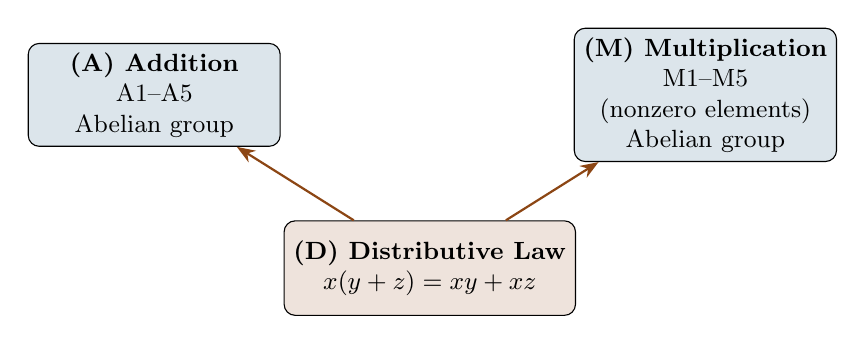
\begin{tikzpicture}[
    box/.style={draw, rounded corners, minimum width=3.2cm, minimum height=1.2cm, align=center, font=\small},
    >=Stealth
  ]
    \node[box, fill=defcolor!15] (A) at (-3.5,0) {\textbf{(A) Addition}\\A1--A5\\Abelian group};
    \node[box, fill=defcolor!15] (M) at (3.5,0) {\textbf{(M) Multiplication}\\M1--M5\\(nonzero elements)\\Abelian group};
    \node[box, fill=mAccent!15] (D) at (0,-2.2) {\textbf{(D) Distributive Law}\\$x(y+z) = xy + xz$};
    \draw[->, thick, mAccent] (D) -- (A);
    \draw[->, thick, mAccent] (D) -- (M);
  \end{tikzpicture}
  \end{center}

  \note{
    This diagram summarizes the structure of the field axioms. On the left
    we have the five addition axioms, which make the set an abelian group
    under addition. On the right, the five multiplication axioms make the
    nonzero elements an abelian group under multiplication. The distributive
    law at the bottom is the bridge connecting the two operations into a
    single coherent structure. Next, let's note some useful conventions
    and examples.
  }
\end{frame}

% =============================================================================
% SECTION: REMARKS AND NOTATION
% =============================================================================

\section{Remarks and Notation}

% --- Remark 1.13(a) ---
\begin{frame}{Remarks 1.13: Shorthand Notation}
  \begin{remblock}{Remark 1.13(a): Notation}
    In any field, we write:
    \[
      x - y \;\text{ for }\; x + (-y), \qquad \frac{x}{y} \;\text{ for }\; x \cdot \frac{1}{y}
    \]
    \[
      x^2 \;\text{ for }\; xx, \qquad 2x \;\text{ for }\; x + x, \qquad \text{etc.}
    \]
  \end{remblock}

  \note{
    Remark 1.13 part "a" introduces the standard shorthand notations we use
    in fields. Subtraction is defined as adding the additive inverse, and
    division is defined as multiplying by the multiplicative inverse.
    Similarly, "x" squared means "x" times x, and 2 "x" means "x" plus x. These
    are all abbreviations built from the two basic operations. With this
    notation in hand, let's see the most important example of a field.
  }
\end{frame}

% --- Remark 1.13(b) ---
\begin{frame}{Remarks 1.13: $\mathbb{Q}$ Is a Field}
  \begin{remblock}{Remark 1.13(b)}
    The rational numbers $\mathbb{Q}$, with the usual addition and multiplication, form a \alert{field}.
  \end{remblock}

  \vspace{0.5em}
  All ten axioms (A1)--(A5), (M1)--(M5), and (D) hold in $\mathbb{Q}$.

  \note{
    The most familiar example of a field is the set of rational numbers "Q".
    All the field axioms hold for the rationals with their customary
    addition and multiplication. So "Q" is a field, and everything we prove
    about fields in general will automatically apply to the rationals.
  }
\end{frame}

% --- Remark 1.13(c) ---
\begin{frame}{Remarks 1.13: Why Study Fields?}
  \begin{remblock}{Remark 1.13(c)}
    Familiar properties of $\mathbb{Q}$ are \emph{consequences} of the field axioms.
  \end{remblock}

  \vspace{0.5em}
  \textbf{Key insight:} Proving results at the field level means we get them
  \alert{for free} in $\mathbb{Q}$, $\mathbb{R}$, and $\mathbb{C}$.

  \note{
    Part "c" of Remark 1.13 explains why we bother with this abstract setup.
    Many familiar properties of the rationals, such as cancellation laws
    and sign rules, are actually consequences of the field axioms alone.
    Once we prove them at this level of generality, we will not need to
    reprove them when we construct the real numbers or the complex numbers.
    Let's now see what the field axioms imply.
  }
\end{frame}

% =============================================================================
% SECTION: CONSEQUENCES OF THE AXIOMS
% =============================================================================

\section{Consequences of the Field Axioms}

% --- Proposition 1.14: Statement Build 1/2 ---
\begin{frame}{Proposition 1.14: Cancellation Laws for Addition}
  \begin{thmblock}{Proposition 1.14}
    The axioms for addition imply:
    \begin{itemize}
      \item[(a)] If $x + y = x + z$ then $y = z$ \hfill \emph{(cancellation law)}
      \item[(b)] If $x + y = x$ then $y = 0$ \hfill \emph{(uniqueness of $0$)}
    \end{itemize}
  \end{thmblock}

  \note{
    Proposition 1.14 lists four consequences of the addition axioms. Part "a"
    is the cancellation law for addition: if "x" plus "y" equals "x" plus z, then
    "y" must equal z. Part "b" says that the additive identity zero is unique.
    If adding "y" to "x" gives back x, then "y" must be zero.
  }
\end{frame}

% --- Proposition 1.14: Statement Build 2/2 ---
\begin{frame}{Proposition 1.14: Cancellation Laws for Addition}
  \begin{thmblock}{Proposition 1.14}
    The axioms for addition imply:
    \begin{itemize}
      \item[(a)] If $x + y = x + z$ then $y = z$ \hfill \emph{(cancellation law)}
      \item[(b)] If $x + y = x$ then $y = 0$ \hfill \emph{(uniqueness of $0$)}
      \item[(c)] If $x + y = 0$ then $y = -x$ \hfill \emph{(uniqueness of $-x$)}
      \item[(d)] $-(-x) = x$ \hfill \emph{(double negation)}
    \end{itemize}
  \end{thmblock}

  \note{
    Part "c" says the additive inverse is unique: the only element that sums
    with "x" to give zero is negative "x". And part "d" is the double negation
    law: negating "x" twice gives back "x". Let's prove these statements.
  }
\end{frame}

% --- Proof of 1.14: Strategy ---
\begin{frame}{Proof of Proposition 1.14 --- Strategy}
  \textbf{Goal:} Prove (a), then derive (b), (c), (d) from (a).

  \vspace{1em}
  \textbf{Key idea for (a):} Add $-x$ to both sides and use the axioms to simplify.

  \vspace{1em}
  \begin{center}
  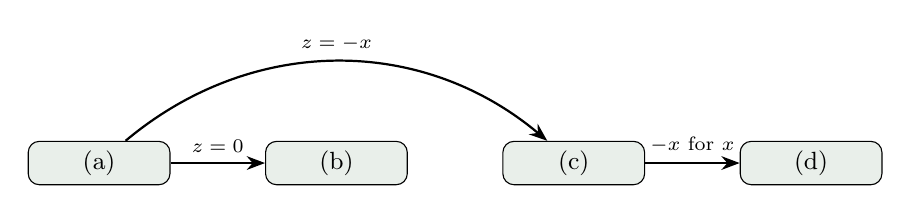
\begin{tikzpicture}[
    node distance=1.2cm,
    box/.style={draw, rounded corners, fill=proofcolor!10, minimum width=1.8cm, font=\small},
    >=Stealth
  ]
    \node[box] (a) {(a)};
    \node[box, right=of a] (b) {(b)};
    \node[box, right=of b] (c) {(c)};
    \node[box, right=of c] (d) {(d)};
    \draw[->, thick] (a) -- node[above, font=\scriptsize]{$z=0$} (b);
    \draw[->, thick] (a) to[bend left=40] node[above, font=\scriptsize]{$z=-x$} (c);
    \draw[->, thick] (c) -- node[above, font=\scriptsize]{$-x$ for $x$} (d);
  \end{tikzpicture}
  \end{center}

  \note{
    Before we dive into the details, let's see the big picture. The core
    result is part "a", the cancellation law. Once we have that, parts "b", "c",
    and "d" follow as special cases. Part "b" comes from setting "z" equal to
    zero in part "a". Part "c" comes from setting "z" equal to negative "x". And
    part "d" follows from part "c" by replacing "x" with negative "x". So the real
    work is in proving part "a".
  }
\end{frame}

% --- Proof of 1.14(a): The chain of equalities ---
\begin{frame}{Proof of Proposition 1.14(a)}
  \begin{proofblock}{Proof of (a): If $x + y = x + z$ then $y = z$}
    Assume $x + y = x + z$. Then:
    \begin{align*}
      y &= 0 + y              & &\text{by (A4)} \\
        &= (-x + x) + y       & &\text{by (A5)} \\
        &= -x + (x + y)       & &\text{by (A3)} \\
        &= -x + (x + z)       & &\text{by hypothesis} \\
        &= (-x + x) + z       & &\text{by (A3)} \\
        &= 0 + z = z           & &\text{by (A5), (A4)}
    \end{align*}
  \end{proofblock}

  \note{
    Here is the proof of part "a". We start with "y", rewrite 0 as negative "x"
    plus "x" using axiom A5, then use associativity to regroup. At the
    crucial step, we swap "x" plus "y" for "x" plus "z" using our hypothesis. Then
    we regroup again and simplify using A5 and A4 to get "z". Every step
    uses only the addition axioms and the hypothesis.
  }
\end{frame}

% --- Proof of 1.14(b)-(d) ---
\begin{frame}{Proof of Proposition 1.14(b)--(d)}
  \small
  \begin{thmblock}{Recall 1.14}
    \begin{tabular}{@{}l@{\qquad}l@{}}
      (a) $x + y = x + z \Rightarrow y = z$ & (c) $x + y = 0 \Rightarrow y = -x$ \\[2pt]
      (b) $x + y = x \Rightarrow y = 0$     & (d) $-(-x) = x$
    \end{tabular}
  \end{thmblock}

  \vspace{0.3em}
  \begin{proofblock}{Deriving (b), (c), (d) from (a)}
    \begin{itemize}
      \item \textbf{(b):} $x + y = x = x + 0$, so $y = 0$ by (a) with $z = 0$
      \item \textbf{(c):} $x + y = 0 = x + (-x)$, so $y = -x$ by (a) with $z = -x$
      \item \textbf{(d):} $(-x) + x = 0$, so by (c) with $-x$ for $x$: $-(-x) = x$
    \end{itemize}
  \end{proofblock}

  \note{
    Parts "b" through "d" all follow from the cancellation law. For part "b",
    the equation "x" plus "y" equals "x" is the same as "x" plus "y" equals "x" plus
    zero, so "y" equals zero by cancellation. For part "c", "x" plus "y" equals
    zero is the same as "x" plus "y" equals "x" plus negative "x", so "y" equals
    negative "x". For part "d", we know negative "x" plus "x" equals zero, and
    by part "c" this means the element that sums with negative "x" to give
    zero must be "x", so the negative of negative "x" is "x".
  }
\end{frame}

% --- Proposition 1.15: Statement ---
\begin{frame}{Proposition 1.15: Cancellation Laws for Multiplication}
  \begin{thmblock}{Proposition 1.15}
    The axioms for multiplication imply (for $x \neq 0$):
    \begin{itemize}
      \item[(a)] If $xy = xz$ then $y = z$ \hfill \emph{(cancellation law)}
      \item[(b)] If $xy = x$ then $y = 1$ \hfill \emph{(uniqueness of $1$)}
      \item[(c)] If $xy = 1$ then $y = 1/x$ \hfill \emph{(uniqueness of $1/x$)}
      \item[(d)] $1/(1/x) = x$ \hfill \emph{(double inversion)}
    \end{itemize}
  \end{thmblock}

  \note{
    Proposition 1.15 states the exact same cancellation laws, but for
    multiplication instead of addition. The requirement that "x" is nonzero
    is essential, since zero does not have a multiplicative inverse. The
    proof follows the same pattern as the proof of Proposition 1.14: prove
    part "a" by multiplying both sides by 1 over x, then derive the rest as
    special cases. Rudin omits the proof because it is so similar. Let's
    see the analogy more clearly on the next slide.
  }
\end{frame}

% --- Proposition 1.14 vs 1.15: Parallel Structure ---
\begin{frame}{Propositions 1.14 and 1.15: The Parallel Structure}
  \begin{center}
  \footnotesize
  \renewcommand{\arraystretch}{1.3}
  \begin{tabular}{c|cc}
    & \textbf{Addition (1.14)} & \textbf{Multiplication (1.15)} \\
    \hline
    Identity & $0$ & $1$ \\
    Inverse & $-x$ & $1/x$ \;\emph{($x \neq 0$)} \\
    \hline
    (a) Cancel & $x{+}y = x{+}z \Rightarrow y{=}z$ & $xy = xz \Rightarrow y{=}z$ \\
    (b) Unique id & $x{+}y = x \Rightarrow y{=}0$ & $xy = x \Rightarrow y{=}1$ \\
    (c) Unique inv & $x{+}y = 0 \Rightarrow y{=}{-x}$ & $xy = 1 \Rightarrow y{=}1/x$ \\
    (d) Double inv & $-(-x) = x$ & $1/(1/x) = x$ \\
  \end{tabular}
  \end{center}

  \note{
    This table makes the parallel between Propositions 1.14 and 1.15 explicit.
    Every statement about addition has an exact counterpart for multiplication.
    You just replace plus with times, zero with one, and negative "x" with 1 over
    x. The only difference is that the multiplication versions require "x" to be
    nonzero, since zero has no multiplicative inverse. This symmetry is not a
    coincidence: both addition and multiplication give abelian groups, so they
    satisfy the same abstract cancellation laws. Now let's see what happens
    when we use both operations together.
  }
\end{frame}

% --- Proposition 1.16: Statement Build 1/2 ---
\begin{frame}{Proposition 1.16: Further Consequences}
  \begin{thmblock}{Proposition 1.16}
    The field axioms imply, for any $x, y, z \in F$:
    \begin{itemize}
      \item[(a)] $0x = 0$
      \item[(b)] If $x \neq 0$ and $y \neq 0$ then $xy \neq 0$
    \end{itemize}
  \end{thmblock}

  \note{
    Proposition 1.16 gives four more consequences of the full field axioms.
    Part "a" says that zero times anything is zero. This seems obvious, but
    it actually requires proof because the axioms only tell us about the
    additive role of zero, not about what happens when we multiply by it.
    Part "b" says a product of nonzero elements is nonzero. This is
    sometimes called the absence of zero divisors. Two more consequences
    are coming next.
  }
\end{frame}

% --- Proposition 1.16: Statement Build 2/2 ---
\begin{frame}{Proposition 1.16: Further Consequences}
  \begin{thmblock}{Proposition 1.16}
    The field axioms imply, for any $x, y, z \in F$:
    \begin{itemize}
      \item[(a)] $0x = 0$
      \item[(b)] If $x \neq 0$ and $y \neq 0$ then $xy \neq 0$
      \item[(c)] $(-x)y = -(xy) = x(-y)$
      \item[(d)] $(-x)(-y) = xy$
    \end{itemize}
  \end{thmblock}

  \note{
    Part "c" is the sign rule for products: negative "x" times "y" equals the
    negative of "x" times y, and the same holds if we negate "y" instead.
    Part "d" says that negating both factors leaves the product unchanged.
    Let's prove each of these.
  }
\end{frame}

% --- Proof of 1.16(a) ---
\begin{frame}{Proof of Proposition 1.16(a): $0x = 0$}
  {\small\colorbox{thmcolor!8}{\strut\;%
    \textbf{Recall 1.14(b):} $x + y = x \;\Rightarrow\; y = 0$%
  \;\;}}

  \vspace{0.3em}
  \begin{proofblock}{Proof of (a)}
    \[
      0x + 0x = (0 + 0)x = 0x
    \]
    By 1.14(b): $\quad 0x = 0$ \qquad $\boxed{0x = 0}$
  \end{proofblock}

  \vspace{0.3em}
  \textbf{Key idea:} Use the distributive law to turn $0 = 0 + 0$ into a statement about products.

  \note{
    The proof of part "a" is elegant and short. We use the fact that zero
    plus zero equals zero, which is just axiom A4. Multiplying both sides
    by "x" and applying the distributive law gives 0 "x" plus 0 "x" equals 0 "x".
    Now recall Proposition 1.14 part "b", which says that if "x" plus "y"
    equals "x", then "y" must be zero. Here, 0 "x" plays the role of both "x" and
    "y", so 0 "x" must be zero.
    This is the first time we have used the distributive law, and it is
    the bridge that lets us connect the additive property of zero with
    multiplication.
  }
\end{frame}

% --- Proof of 1.16(b) ---
\begin{frame}{Proof of Proposition 1.16(b): No Zero Divisors}
  \begin{proofblock}{Proof of (b)}
    \textbf{Assume} $x \neq 0$, $y \neq 0$, but suppose $xy = 0$. Then:
    \[
      1 = \frac{1}{y} \cdot \frac{1}{x} \cdot xy = \frac{1}{y} \cdot \frac{1}{x} \cdot 0 = 0
    \]
    This gives $1 = 0$, \alert{contradicting} axiom (M4).
  \end{proofblock}

  \note{
    For part "b", we use proof by contradiction. Suppose "x" and "y" are both
    nonzero but their product is zero. Since "x" and "y" are nonzero, their
    multiplicative inverses exist. Multiplying both sides of "x" "y" equals
    zero by 1 over "y" times 1 over "x", the left side simplifies to 1, while
    the right side is zero by part "a". So we get 1 equals 0, which
    contradicts axiom M4. Therefore the product "x" "y" cannot be zero.
  }
\end{frame}

% --- Proof of 1.16(c) ---
\begin{frame}{Proof of Proposition 1.16(c): $(-x)y = -(xy)$}
  {\small\colorbox{thmcolor!8}{\strut\;%
    \textbf{Recall 1.14(c):} $x + y = 0 \;\Rightarrow\; y = -x$%
  \;\;}}

  \vspace{0.3em}
  \begin{proofblock}{Proof of (c)}
    Compute:
    \[
      (-x)y + xy = (-x + x)y = 0y = 0
    \]
    By 1.14(c): $\quad (-x)y = -(xy)$

    \vspace{0.3em}
    Similarly: $\; x(-y) + xy = x(-y + y) = x \cdot 0 = 0$, so $x(-y) = -(xy)$.
  \end{proofblock}

  \note{
    To prove that negative "x" times "y" equals negative of "x" "y", we show that
    their sum with "x" "y" is zero. By the distributive law, negative "x" times
    "y" plus "x" times "y" equals the quantity negative "x" plus "x" times "y", which
    is zero times "y", which is zero by part "a". Now recall Proposition 1.14
    part "c", which says that if "x" plus "y" equals zero, then "y" is the
    additive inverse of "x". Applying that here, negative "x" times "y" must be
    the additive inverse of "x" "y". The second equality follows by the same
    argument with "y" negated instead.
  }
\end{frame}

% --- Proof of 1.16(d) ---
\begin{frame}{Proof of Proposition 1.16(d): $(-x)(-y) = xy$}
  {\small\colorbox{thmcolor!8}{\strut\;%
    \textbf{Recall 1.16(c):} $(-x)y = -(xy)$%
  \;\;}\quad\colorbox{thmcolor!8}{\strut\;%
    \textbf{Recall 1.14(d):} $-(-x) = x$%
  \;\;}}

  \vspace{0.3em}
  \begin{proofblock}{Proof of (d)}
    By 1.16(c) and 1.14(d):
    \[
      (-x)(-y) = -\bigl[x(-y)\bigr] = -\bigl[-(xy)\bigr] = xy
    \]
    $\boxed{(-x)(-y) = xy}$
  \end{proofblock}

  \vspace{0.5em}
  The product of two negated elements equals the product of the originals --- not by convention, but by \alert{proof}.

  \note{
    Part "d" follows from two applications of what we have already proved.
    Recall that part "c" tells us that negating one factor is the same as
    negating the whole product. By part "c", negative "x" times negative "y"
    equals the negative of "x" times negative "y". Applying part "c" again, "x"
    times negative "y" is the negative of "x" "y". So we have the negative of
    the negative of "x" "y". And recall Proposition 1.14 part "d", the double
    negation law, which says the negative of the negative of "x" "y" is just
    "x" "y". Notice that this result holds
    in any field, not just ordered fields. We have not used any notion
    of positivity here, only the algebraic axioms. The familiar sign
    rule from arithmetic is a purely algebraic consequence. Now let's
    add order structure to our fields.
  }
\end{frame}

% =============================================================================
% SECTION: ORDERED FIELDS
% =============================================================================

\section{Ordered Fields}

% --- Definition 1.17 ---
\begin{frame}{Definition 1.17: Ordered Field}
  \begin{defblock}{Definition 1.17}
    An \alert{ordered field} is a field $F$ that is also an ordered set, such that:
    \begin{itemize}
      \item[(i)] $y < z \;\Longrightarrow\; x + y < x + z$ \hfill \emph{(order + addition)}
      \item[(ii)] $x > 0$ and $y > 0 \;\Longrightarrow\; xy > 0$ \hfill \emph{(order + multiplication)}
    \end{itemize}
  \end{defblock}

  \vspace{0.5em}
  If $x > 0$: \emph{positive}. \quad If $x < 0$: \emph{negative}.

  \vspace{0.3em}
  \textbf{Example:} $\mathbb{Q}$ is an ordered field.

  \note{
    An ordered field combines the algebraic structure of a field with the
    order structure from the previous section. Two compatibility conditions
    are required. First, adding the same element to both sides of an
    inequality preserves the inequality. Second, the product of two
    positive elements is positive. Elements greater than zero are called
    positive, and elements less than zero are called negative. The
    rationals "Q" are the primary example of an ordered field we have seen
    so far.
  }
\end{frame}

% --- Diagram: Ordered Field Structure ---
\begin{frame}{Ordered Field = Field + Compatible Order}
  \begin{center}
  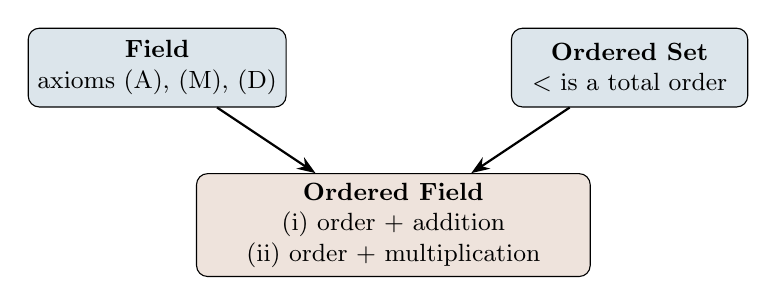
\begin{tikzpicture}[
    box/.style={draw, rounded corners, minimum width=3cm, minimum height=1cm, align=center, font=\small},
    >=Stealth
  ]
    \node[box, fill=defcolor!15] (F) at (-3,0.8) {\textbf{Field}\\axioms (A), (M), (D)};
    \node[box, fill=defcolor!15] (O) at (3,0.8) {\textbf{Ordered Set}\\$<$ is a total order};
    \node[box, fill=mAccent!15, minimum width=5cm] (OF) at (0,-1.2) {\textbf{Ordered Field}\\(i) order + addition\\(ii) order + multiplication};
    \draw[->, thick] (F) -- (OF);
    \draw[->, thick] (O) -- (OF);
  \end{tikzpicture}
  \end{center}

  \note{
    This diagram shows how the concept of an ordered field brings together
    two structures we have already defined: a field and an ordered set.
    The two compatibility conditions, shown in the box at the bottom,
    ensure that the algebraic operations respect the ordering. This
    combined structure is what allows us to work with both equations and
    inequalities in a consistent way. Let's see what these compatibility
    conditions look like. Let's see what properties follow.
  }
\end{frame}

% --- Proposition 1.18: Statement Build 1/3 ---
\begin{frame}{Proposition 1.18: Properties of Ordered Fields}
  \begin{thmblock}{Proposition 1.18}
    In every ordered field:
    \begin{itemize}
      \item[(a)] If $x > 0$ then $-x < 0$, and vice versa
      \item[(b)] If $x > 0$ and $y < z$ then $xy < xz$
    \end{itemize}
  \end{thmblock}

  \note{
    Proposition 1.18 lists the fundamental properties of ordered fields.
    Part "a" says that positive and negative are linked through negation:
    the negative of a positive number is negative, and vice versa. Part "b"
    says that multiplying an inequality by a positive number preserves the
    direction of the inequality. But what happens when we multiply by a
    negative number?
  }
\end{frame}

% --- Proposition 1.18: Statement Build 2/3 ---
\begin{frame}{Proposition 1.18: Properties of Ordered Fields}
  \begin{thmblock}{Proposition 1.18}
    In every ordered field:
    \begin{itemize}
      \item[(a)] If $x > 0$ then $-x < 0$, and vice versa
      \item[(b)] If $x > 0$ and $y < z$ then $xy < xz$
      \item[(c)] If $x < 0$ and $y < z$ then $xy > xz$
    \end{itemize}
  \end{thmblock}

  \note{
    Part "c" is the complementary rule: multiplying by a negative number
    reverses the inequality. This is the familiar rule that multiplying
    both sides of an inequality by a negative flips the direction. Two
    more properties round out the picture.
  }
\end{frame}

% --- Proposition 1.18: Statement Build 3/3 ---
\begin{frame}{Proposition 1.18: Properties of Ordered Fields}
  \begin{thmblock}{Proposition 1.18}
    In every ordered field:
    \begin{itemize}
      \item[(a)] If $x > 0$ then $-x < 0$, and vice versa
      \item[(b)] If $x > 0$ and $y < z$ then $xy < xz$
      \item[(c)] If $x < 0$ and $y < z$ then $xy > xz$
      \item[(d)] If $x \neq 0$ then $x^2 > 0$. In particular, $1 > 0$
      \item[(e)] If $0 < x < y$ then $0 < 1/y < 1/x$
    \end{itemize}
  \end{thmblock}

  \note{
    Part "d" tells us that every nonzero square is positive, and since 1
    equals 1 squared, we get that 1 is positive. Part "e" says that taking
    reciprocals of positive numbers reverses their order. These are all
    rules you have used many times, and now we will prove them rigorously
    from the axioms.
  }
\end{frame}

% --- Proof of 1.18(a) ---
\begin{frame}{Proof of Proposition 1.18(a)}
  \begin{proofblock}{Proof of (a): $x > 0 \;\Longrightarrow\; -x < 0$}
    If $x > 0$, add $-x$ to both sides of $0 < x$ using 1.17(i):
    \[
      -x = -x + 0 < -x + x = 0
    \]
    so $-x < 0$. If $x < 0$, the same argument gives $-x > 0$.
  \end{proofblock}

  \begin{center}
  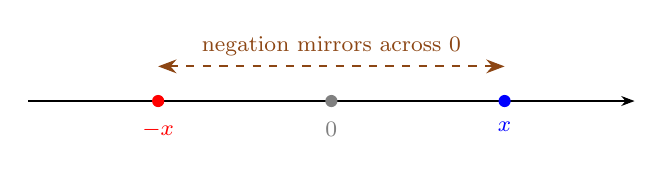
\begin{tikzpicture}[>=Stealth, scale=1.1]
    \draw[->] (-3.5,0) -- (3.5,0);
    \fill[gray] (0,0) circle (2pt) node[below=4pt, font=\footnotesize]{$0$};
    \fill[red] (-2,0) circle (2pt) node[below=4pt, font=\footnotesize]{$-x$};
    \fill[blue] (2,0) circle (2pt) node[below=4pt, font=\footnotesize]{$x$};
    \draw[<->, thick, mAccent, dashed] (-2,0.4) -- (2,0.4)
      node[midway, above, font=\footnotesize]{negation mirrors across $0$};
  \end{tikzpicture}
  \end{center}

  \note{
    To prove part "a", suppose "x" is positive, meaning 0 is less than "x".
    By Definition 1.17 part i, we can add negative "x" to both sides of
    the inequality 0 less than "x". On the left, negative "x" plus 0 equals
    negative "x". On the right, negative "x" plus "x" equals 0. So we get
    negative "x" is less than 0, which means negative "x" is negative. The
    converse direction, that if "x" is negative then negative "x" is positive,
    works the same way: start from "x" less than 0 and add negative "x" to
    both sides. Let's continue with part "b".
  }
\end{frame}

% --- Proof of 1.18(b) ---
\begin{frame}{Proof of Proposition 1.18(b)}
  \begin{proofblock}{Proof of (b): $x > 0,\; y < z \;\Longrightarrow\; xy < xz$}
    Since $z > y$:
    \[
      z - y > y - y = 0
    \]
    so $z - y > 0$. Since $x > 0$, Definition 1.17(ii) gives $x(z - y) > 0$. Therefore:
    \[
      xz = x(z-y) + xy > 0 + xy = xy
    \]
    $\boxed{xy < xz}$
  \end{proofblock}

  \note{
    For part "b", we need to show that multiplying a strict inequality by a
    positive number preserves the direction. Since "z" is greater than "y",
    "z" minus "y" is positive. Multiplying two positive numbers, "x" and "z" minus
    "y", gives a positive product. So "x" times "z" minus "y" is positive, which
    means "x" "z" is greater than "x" "y". This is exactly the rule we wanted.
    Next, let's handle the case of multiplying by a negative.
  }
\end{frame}

% --- Proof of 1.18(c) ---
\begin{frame}{Proof of Proposition 1.18(c)}
  {\small\colorbox{thmcolor!8}{\strut\;%
    \textbf{Recall 1.16(c):} $(-x)y = -(xy)$%
  \;\;}}

  \vspace{0.3em}
  \begin{proofblock}{Proof of (c): $x < 0,\; y < z \;\Longrightarrow\; xy > xz$}
    By (a), $-x > 0$. By 1.16(c):
    \[
      -[x(z - y)] = (-x)(z - y) > 0
    \]
    so $x(z-y) < 0$, hence $xz < xy$.
    $\qquad\boxed{xy > xz}$
  \end{proofblock}

  \note{
    Part "c" handles the case where we multiply by a negative number. Since
    "x" is negative, negative "x" is positive by part "a". Since "y" is less than
    "z", "z" minus "y" is positive. So the product of negative "x" and "z" minus "y"
    is positive by
    the ordered field axiom. Using the sign rule from Proposition 1.16
    part "c", this means the negative of "x" times "z" minus "y" is positive,
    so "x" times "z" minus "y" is negative, meaning "x" "z" is less than "x" "y". The
    inequality is reversed. Now let's prove the result about squares.
  }
\end{frame}

% --- Proof of 1.18(d) ---
\begin{frame}{Proof of Proposition 1.18(d)}
  {\small\colorbox{thmcolor!8}{\strut\;%
    \textbf{Recall 1.16(d):} $(-x)(-y) = xy$%
  \;\;}\quad\colorbox{thmcolor!8}{\strut\;%
    \textbf{1.17(ii):} $x,y > 0 \Rightarrow xy > 0$%
  \;\;}}

  \vspace{0.3em}
  \begin{proofblock}{Proof of (d): $x \neq 0 \;\Longrightarrow\; x^2 > 0$}
    Two cases:
    \begin{itemize}
      \item If $x > 0$: then $x^2 = x \cdot x > 0$ \quad (by 1.17(ii))
      \item If $x < 0$: then $-x > 0$, so $(-x)^2 > 0$. But $(-x)^2 = x^2$ \quad (by 1.16(d))
    \end{itemize}

    \vspace{0.5em}
    Since $1 = 1^2$: $\quad \boxed{1 > 0}$
  \end{proofblock}

  \note{
    Part "d" has two cases. If "x" is positive, then "x" times "x" is the product
    of two positive numbers, which is positive by Definition 1.17 part ii,
    the axiom that says the product of two positive elements is positive.
    If "x" is negative, then negative "x" is positive, so negative "x" squared
    is positive. But recall Proposition 1.16 part "d", which says that
    negative "x" times negative "y" equals "x" "y". Setting "y" equal to "x", we get
    negative "x" squared equals "x" squared. Either way, "x" squared is positive. Since
    1 equals 1 squared, we conclude that 1 is positive. This is a
    remarkable fact: the positivity of 1 is not an axiom, but a
    consequence of the other axioms. One more property to go: reciprocals.
  }
\end{frame}

% --- Proof of 1.18(e) ---
\begin{frame}{Proof of Proposition 1.18(e)}
  \begin{proofblock}{Proof of (e): $0 < x < y \;\Longrightarrow\; 0 < 1/y < 1/x$}
    \textbf{Step 1:} Show $1/y > 0$.
    If $1/y \leq 0$, then since $y > 0$, part (b) gives $y \cdot (1/y) \leq 0$.
    But $y \cdot (1/y) = 1 > 0$ by (d). Contradiction.

    \textbf{Step 2:} Similarly, $1/x > 0$.

    \textbf{Step 3:} Multiply $x < y$ by the positive quantity $\frac{1}{x} \cdot \frac{1}{y}$:
    $\displaystyle\frac{1}{y} < \frac{1}{x}$
    \qquad$\boxed{0 < 1/y < 1/x}$
  \end{proofblock}

  \note{
    For part "e", we first show that 1 over "y" is positive. If 1 over "y"
    were zero or negative, then since "y" is positive, their product "y" times
    1 over "y" would be at most zero by parts "b" and "a". But "y" times 1 over "y"
    equals 1, which is positive by part "d". That is a contradiction, so
    1 over "y" must be positive. The same argument shows 1 over "x"
    is positive. Now, multiplying both sides of "x" less than "y" by the
    positive number 1 over "x" times 1 over "y" preserves the inequality and
    gives us 1 over "y" is less than 1 over "x". Taking reciprocals of
    positive numbers reverses the order.
  }
\end{frame}

% =============================================================================
% SUMMARY
% =============================================================================

% --- Summary Build 1/4 ---
\begin{frame}{Summary}
  \textbf{Key takeaways from this section:}
  \begin{itemize}
    \item A \alert{field} is a set with addition and multiplication satisfying axioms (A), (M), and (D)
  \end{itemize}

  \note{
    Let's review what we covered. A field is a set equipped with addition
    and multiplication that satisfy ten axioms plus the distributive law.
    The addition axioms and multiplication axioms each give the structure
    of an abelian group, and the distributive law connects them.
  }
\end{frame}

% --- Summary Build 2/4 ---
\begin{frame}{Summary}
  \textbf{Key takeaways from this section:}
  \begin{itemize}
    \item A \alert{field} is a set with addition and multiplication satisfying axioms (A), (M), and (D)
    \item Cancellation laws, sign rules, uniqueness of $0$ and $1$ all follow from the axioms
  \end{itemize}

  \note{
    We proved that familiar algebraic properties, such as cancellation
    laws, the uniqueness of zero and one, and sign rules like negative
    times negative equals positive, are all consequences of the field
    axioms. We do not need to re-prove them for each specific field.
  }
\end{frame}

% --- Summary Build 3/4 ---
\begin{frame}{Summary}
  \textbf{Key takeaways from this section:}
  \begin{itemize}
    \item A \alert{field} is a set with addition and multiplication satisfying axioms (A), (M), and (D)
    \item Cancellation laws, sign rules, uniqueness of $0$ and $1$ all follow from the axioms
    \item An \alert{ordered field} adds a compatible total order --- the setting for inequalities
  \end{itemize}

  \note{
    An ordered field combines the field structure with a total order that
    is compatible with both addition and multiplication. This is the
    natural setting for working with inequalities.
  }
\end{frame}

% --- Summary Build 4/4 ---
\begin{frame}{Summary}
  \textbf{Key takeaways from this section:}
  \begin{itemize}
    \item A \alert{field} is a set with addition and multiplication satisfying axioms (A), (M), and (D)
    \item Cancellation laws, sign rules, uniqueness of $0$ and $1$ all follow from the axioms
    \item An \alert{ordered field} adds a compatible total order --- the setting for inequalities
    \item Squares are positive, $1 > 0$, and reciprocals reverse order
  \end{itemize}

  \vspace{1em}
  \textbf{Coming up next:} The Real Field --- constructing $\mathbb{R}$ with the \alert{least upper bound property}.

  \note{
    In every ordered field, nonzero squares are positive, 1 is positive,
    multiplying by a negative reverses inequalities, and taking reciprocals
    of positive numbers reverses their order. In the next section, we will
    construct the real numbers as an ordered field with one crucial extra
    property: the least upper bound property. This is the property that
    fills the gaps in the rationals that we identified in the introduction.
    See you there.
  }
\end{frame}

\end{document}
